\section{Case Study: Super-Store Sales Data Analysis}
\label{sec:store_sales_section}

In order to first demonstrate a generalised application of the \textit{R-K pipeline}, \textit{R-K toolkit} and \textit{R-K WorkBench}, we chose to apply our computational framework on a popular non-physical commercial dataset, that serves as a benchmark for standardization of various analytical tools and softwares in the domains of Data-Science \& Big-Data Analytics. Therefore we shall show the implementation \& applications of our generalised R-K Pipeline to a standard super-store sales dataset released by Tableau.\cite{TableauSuperStore} This dataset was chosen for \textbf{3 primary reasons:}

\begin{enumerate}
        \item{Since the initial analysis was done on LIGO data, we decided to choose an unrelated and orthogonal dataset to prove that the core concepts of the R-K workflow can traverse across domains. The R-K Diagrams are meant to be generalizable across many domains and we wanted to prove it was possible.}
        \item{Store sales require less domain knowledge for demonstration purposes. This makes it an easier dataset to teach the core concepts.}
        \item{It is a widely applied in research and is extremely accessible.A snapshot of the dataset along with the relevant columns for our pipeline is shown in figure \ref{fig:sample store sales dataset} for reference and can be matched to the one released by  Tableau.\cite{TableauSuperStore}}
\end{enumerate}

\begin{figure*}[t]
	\centering
        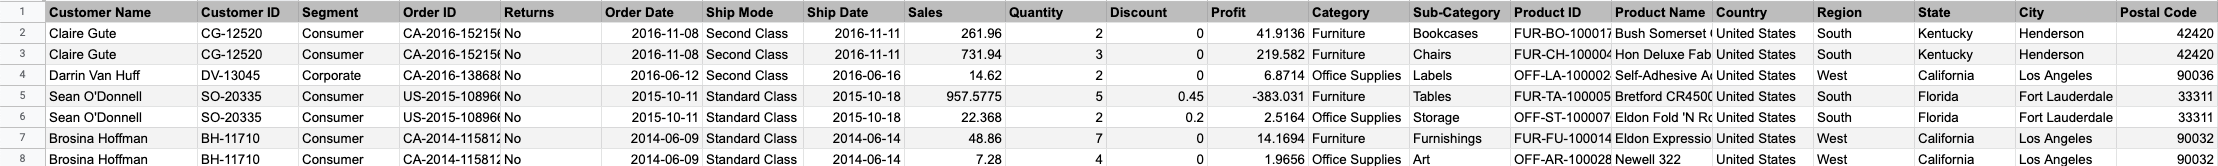
\includegraphics[width=1\textwidth]{images/store_sales_dataset.png}
	\caption{\textit{A Snapshot of the Tableau Super-Store Sales Dataset with the relevant columns which have been modelled via the R-K Pipeline }}
	\label{fig:sample store sales dataset}
\end{figure*}

The corresponding code along with our analytical framework and its applications on this dataset can be found on \href{https://github.com/andorsk/store_sales}{Github}. Our results show that we can generate distinct topological signatures for each transaction event, and that the encoding provides descriptive properties that standard distance evaluation methods would not capture.

\subsection{Data Description}

The data for store sales consisted of the following information: \cite{tableau_community_forums_2021}

\begin{itemize}
        \item Location Data for where the transaction occurred, in the form of country, region, state, city, and postal code.
        \item Identity information such as customer id and segment id.
        \item Information on the order such as the shipment type, returns, shipment date, and shipment mode.
        \item Product information for the line item, specifically the category, sub category, product id, and product name
        \item The information of the sale of the line item: sales, quantity, and discount
\end{itemize}

The data is synthetic data. All data was merged together into a single data-frame within python. The head of the contents can be found below, post merge. The dataset has 9994 entries. A basic description of the numeric entries is available at figure \ref{fig:ssd_stats}. The non-numeric data is preprocessed and encoded into numeric data in the preprocessing step as described in subsection \ref{subsec:Preprocessing}.

\begin{figure}[H]
	\centering
        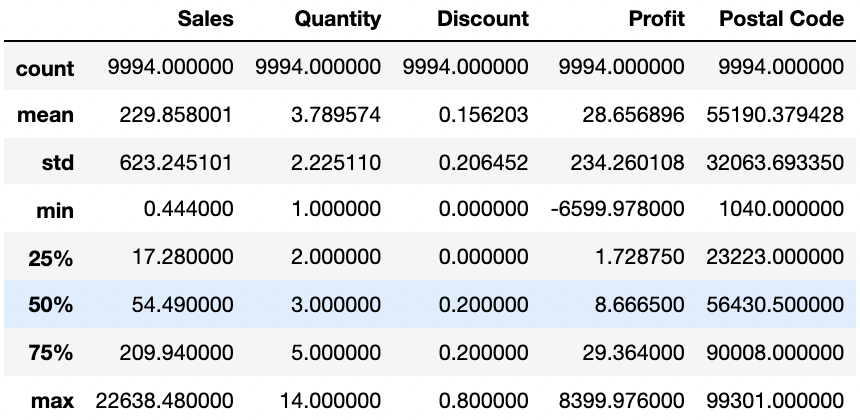
\includegraphics[width=1.0\linewidth]{images/ssd_stats.png}
	\caption{\textit{Summary of the Store Sales Data}}
	\label{fig:ssd_stats}
\end{figure}

\subsection{Objective of Analysis}

The objective of the analysis was to localize and generate R-K Diagrams that provide unique and descriptive topological signature for the data in the form of an R-K Diagram. Through the R-K Pipeline, these structure would preserve a unique topological representations that allows attributive comparisons across events. We expect that the encoding provided through the R-K Pipeline would capture information that normal techniques will fail to capture, and allow for better cross-event comparisons based upon both value and topological distances.

After deriving the unique topological structures, through machine learning, the goal of this analysis is to finally embed the structures in $\mathbb{R}^{2}$ space such that topological differences maximize the inter-R-K Diagram distance and topological similarities minimize the inter-R-K Diagram distance in Phase Space as elaborated subsection \ref{sec:phase_space}.

\subsection{Lens Implementation}

Since R-K-Diagrams represent event based topological signatures, therefore the choice of lens is critical to how the R-K-Diagrams are formed. In this dataset, \textbf{each transaction} was represented as an event. We chose ``transactions'' as an event lens because of the clear use case which represents a discrete temporal purchase event in a sales store. This is demonstrated in figure \ref{fig:lens_choise2} for reference and clarity. It is also important to note that we could have chosen alternative lenses such as a customer, however coercing a customer data source into an event that can be used in the R-K models, involve extracting features from all transaction events of a customer into an ``Customer Observation Event''. Such a use case, while possible, is non-temporal and requires aggregation before applying the lens.

\begin{figure}[H]
    \centering
            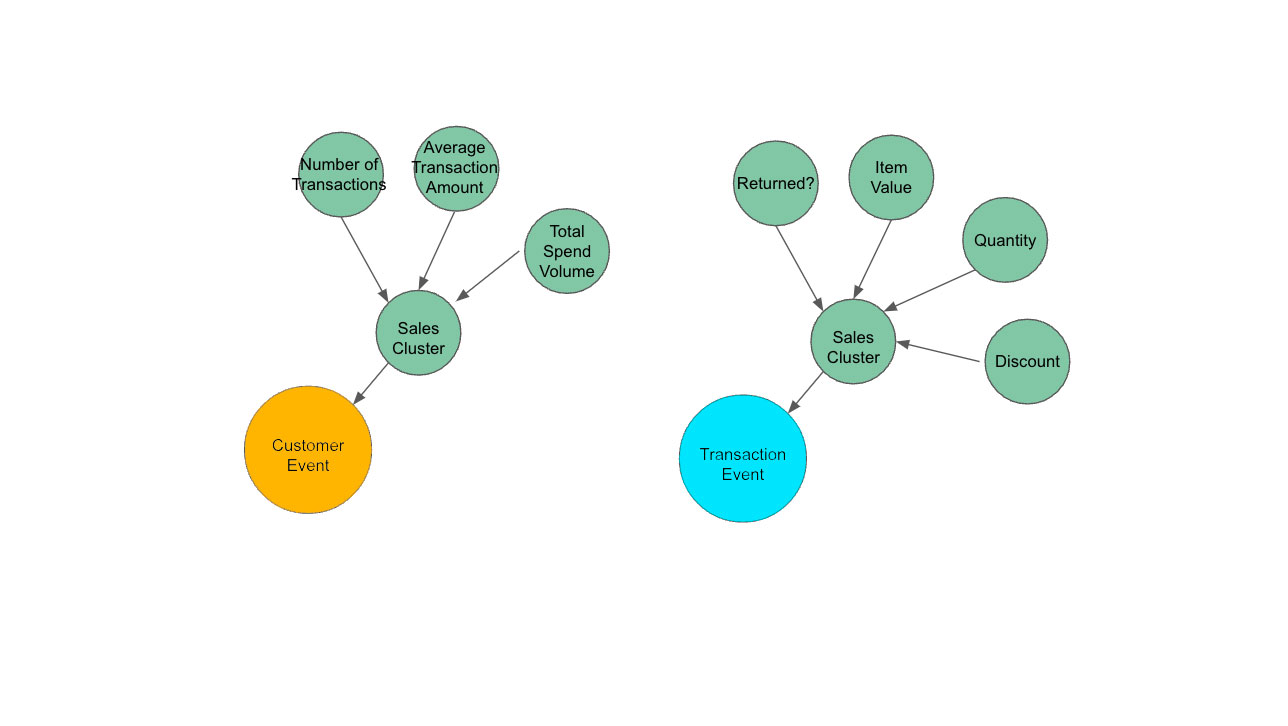
\includegraphics[width=0.5\textwidth]{images/Lens_Choice2.jpg}
    \caption{\textit{The lens choice used for this analysis. We chose to review the data from a transaction level, but various other "lenses" can be applied where appropriate as demonstrated in the diagram above.}}
    \label{fig:lens_choise2}
\end{figure}

\subsection{Preprocessing}
\label{subsec:Preprocessing}
One hot encoding was applied to categorical data. Dates were converted to numbers. Identifiers unique to the event, or with very large cardinality, such as the Customer Id, Product Id, Segment Id, and Product Name, were dropped. Location data was converted into latitudinal and longitudinal positions using Google Map's API's and applying a zip code lookup. Failure to search the latitude and/or longitude of a particular zip resulted in removal from the dataset.

The resulting dataset after transformations became 9918 rows and 90 columns. The data was then normalized over a MinMaxScaler so that training the models were more effective.

\subsection{Deriving the Hierarchical Function}

We generated an ontology based on our domain understanding of store sales data. The graph was documented as a JSON file and provides the \textit{Structure Graph} of the R-K-Diagrams. The ontology was coerced into a transformation node that take in a Pandas dataframe and returns a graph object, with attributes encoded acocording to the event that was sent to the transform.

The hierarchy was derived by utilizing the domain specific ontological graph. An initial ontology was generated based upon correlation parameters in the data-set along with the application of financial domain knowledge on Super Store Sales data. The ontology graphs used or generated for this purpose can be found in the following link: \url{https://github.com/animikhroy/rk_toolkit_pipeline_diagrams/tree/main/02_notebooks/rk_general_applications/data}

\begin{figure}[H]
	\centering
        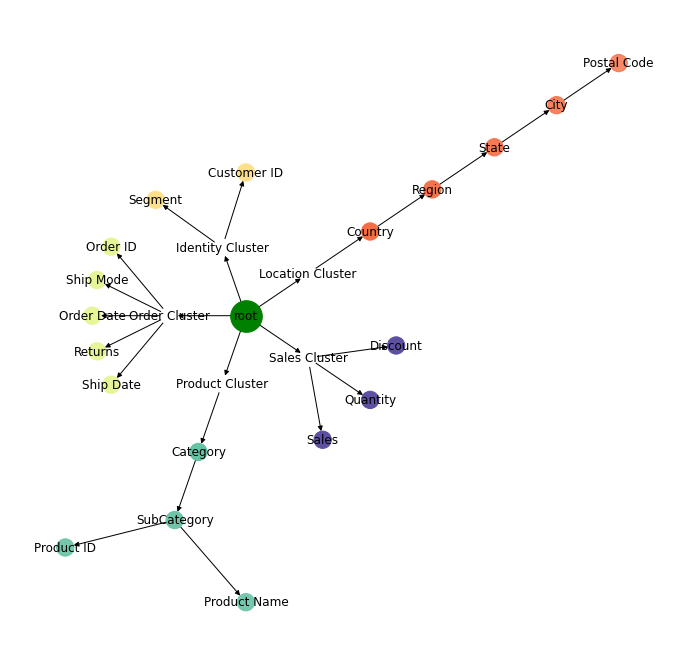
\includegraphics[width=0.5\textwidth]{images/base_hierarchy.png}
	\caption{\textit{The base hierarchy provided for the store sales data}}
	\label{fig:base hierarchy store sales}
\end{figure}

The structural graph is then generated using the base hierarchy provided for the store sales data. After generating this structural graph, it can be visualized using the R-K Toolkit as shown in the figure  \ref{fig:base hierarchy store sales}.

\begin{figure}
	\centering
        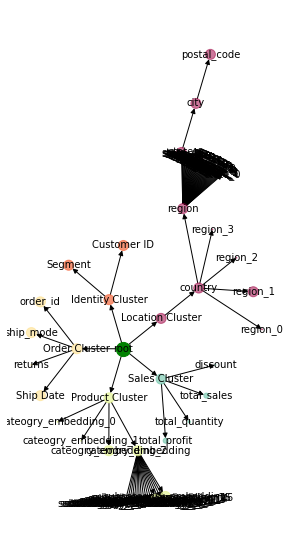
\includegraphics[width=1.0\linewidth]{images/pre-filter-graphs.png}
	\caption{\textit{At the top, you have the core structural graph. Below, are 10 corresponding events without transformation, using the structural graph.  We can see the distance pre-filters and linkages are <metric> where the distance measure is bound between 0 and 1 to evaluate similarity in the R-K pipeline. The distances are purely derived using the value/magnitudinal distance function provided in the R-K toolkit, and the filters and linkage functions that provide topological deviations have not yet been applied at this stage of analysis.}}
	\label{fig:pre-filter-graphs}
\end{figure}

As you can see in figure \ref{fig:pre-filter-graphs}, we have expanded out the original hierarchy with the help of categorical data made available by Tableau. This can be compressed in later steps back to the original form if required using isometric compression techniques available in the R-K Toolkit.

\subsection{Pipeline Construction with Filter and Linker Designs}

We used a basic filter (The RangeFilter) and linker called (SimpleChildLinker) design as explained below.

\subsubsection{RangeFilter}

A range filter is one of the simpliest filters that is provided in version 1 of the R-K Toolkit. We assign the filters to each level of the hierarchy that contains numeric data.

\[
\begin{cases}
   true  & \text{if } v \notin \lbrace m, M \rbrack\\
   false & \text{else}
\end{cases}
\]

where:

\begin{itemize}
        \item{$v$ is the value of the node}
        \item{$m$ is the minimum boundary condition for the filter}
        \item{$M$ is the maximum boundary condition for the filter}
\end{itemize}

\subsubsection{LeafLinker}

We also used the simple leaf linker, which is provided in the R-K Toolkit. The simple leaf linker compares only the leafs of a tree, and provides an edge $E$ in the case the euclidean distance is less than the specified threshold:

\begin{figure}[h]
	\centering
        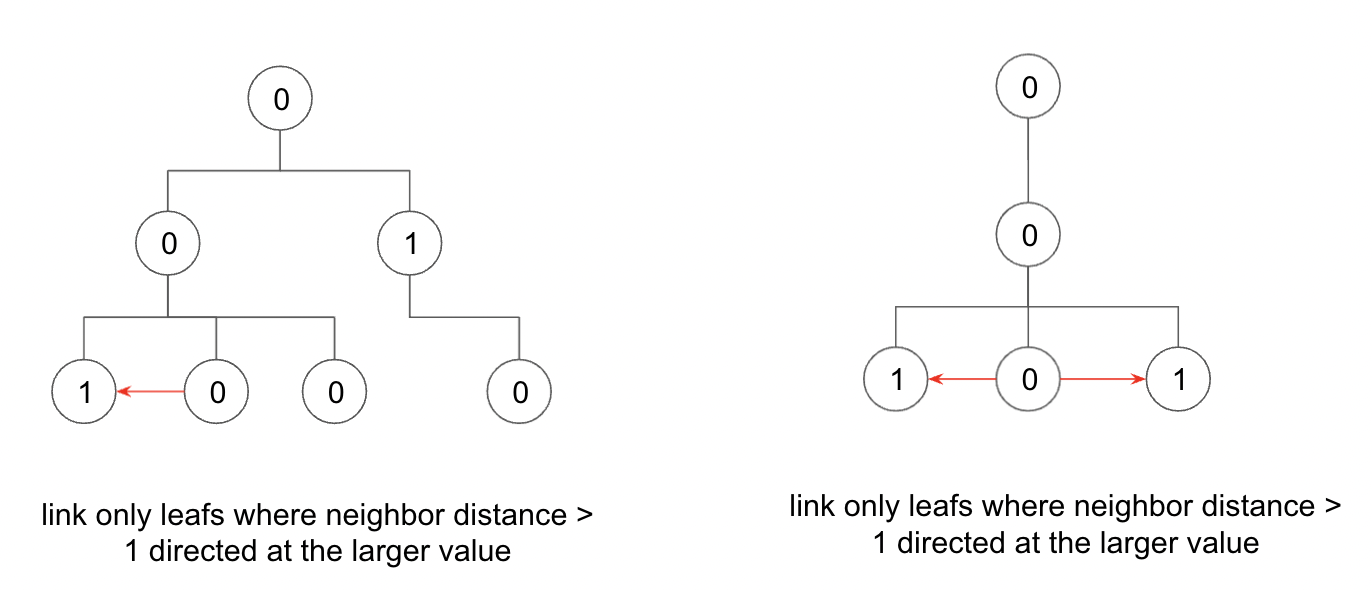
\includegraphics[width=0.5\textwidth]{images/linkage.png}
	\caption{\textit{Leaf Linker compares the distances between values with $\epsilon$ < $\theta$, and links the leafs of the final clusters based upon the threshold.}}
	\label{fig:linkage2}
\end{figure}

Mathematically, this linkage is represented below:
\[
\begin{cases}
     E & \text{if } \epsilon \le \theta\\
     None & \text{else}
\end{cases}
\]


\paragraph{where}
\begin{itemize}
  \item{$n_{i}$ and $n_{j}$ are two leaf nodes }
  \item{$\epsilon = || \sqrt{n_{i}-n_{j}^{2}} ||$}
  \item{$\theta$ is a defined tolerance for linkage}
\end{itemize}

The LeafLinker's O notation would be $O(n^{2})$, however the number of total computations more concretely is $\sum_{i=0}^{i=|C|}\frac{N!}{2(N-2)!}$ where $|C|$ is the number of clusters and $|N|$ is the number of leafs within the cluster.

\subsection{Visualizing an Untrained Network}

The following image below demonstrates the first 10 rows of the store sales data with untrained thresholds.This time the base-structural graph has been updated with appropriate filter and linker functions as described in the previous sections to be able to generate a base R-K Model.

\begin{figure}[H]
	\centering
        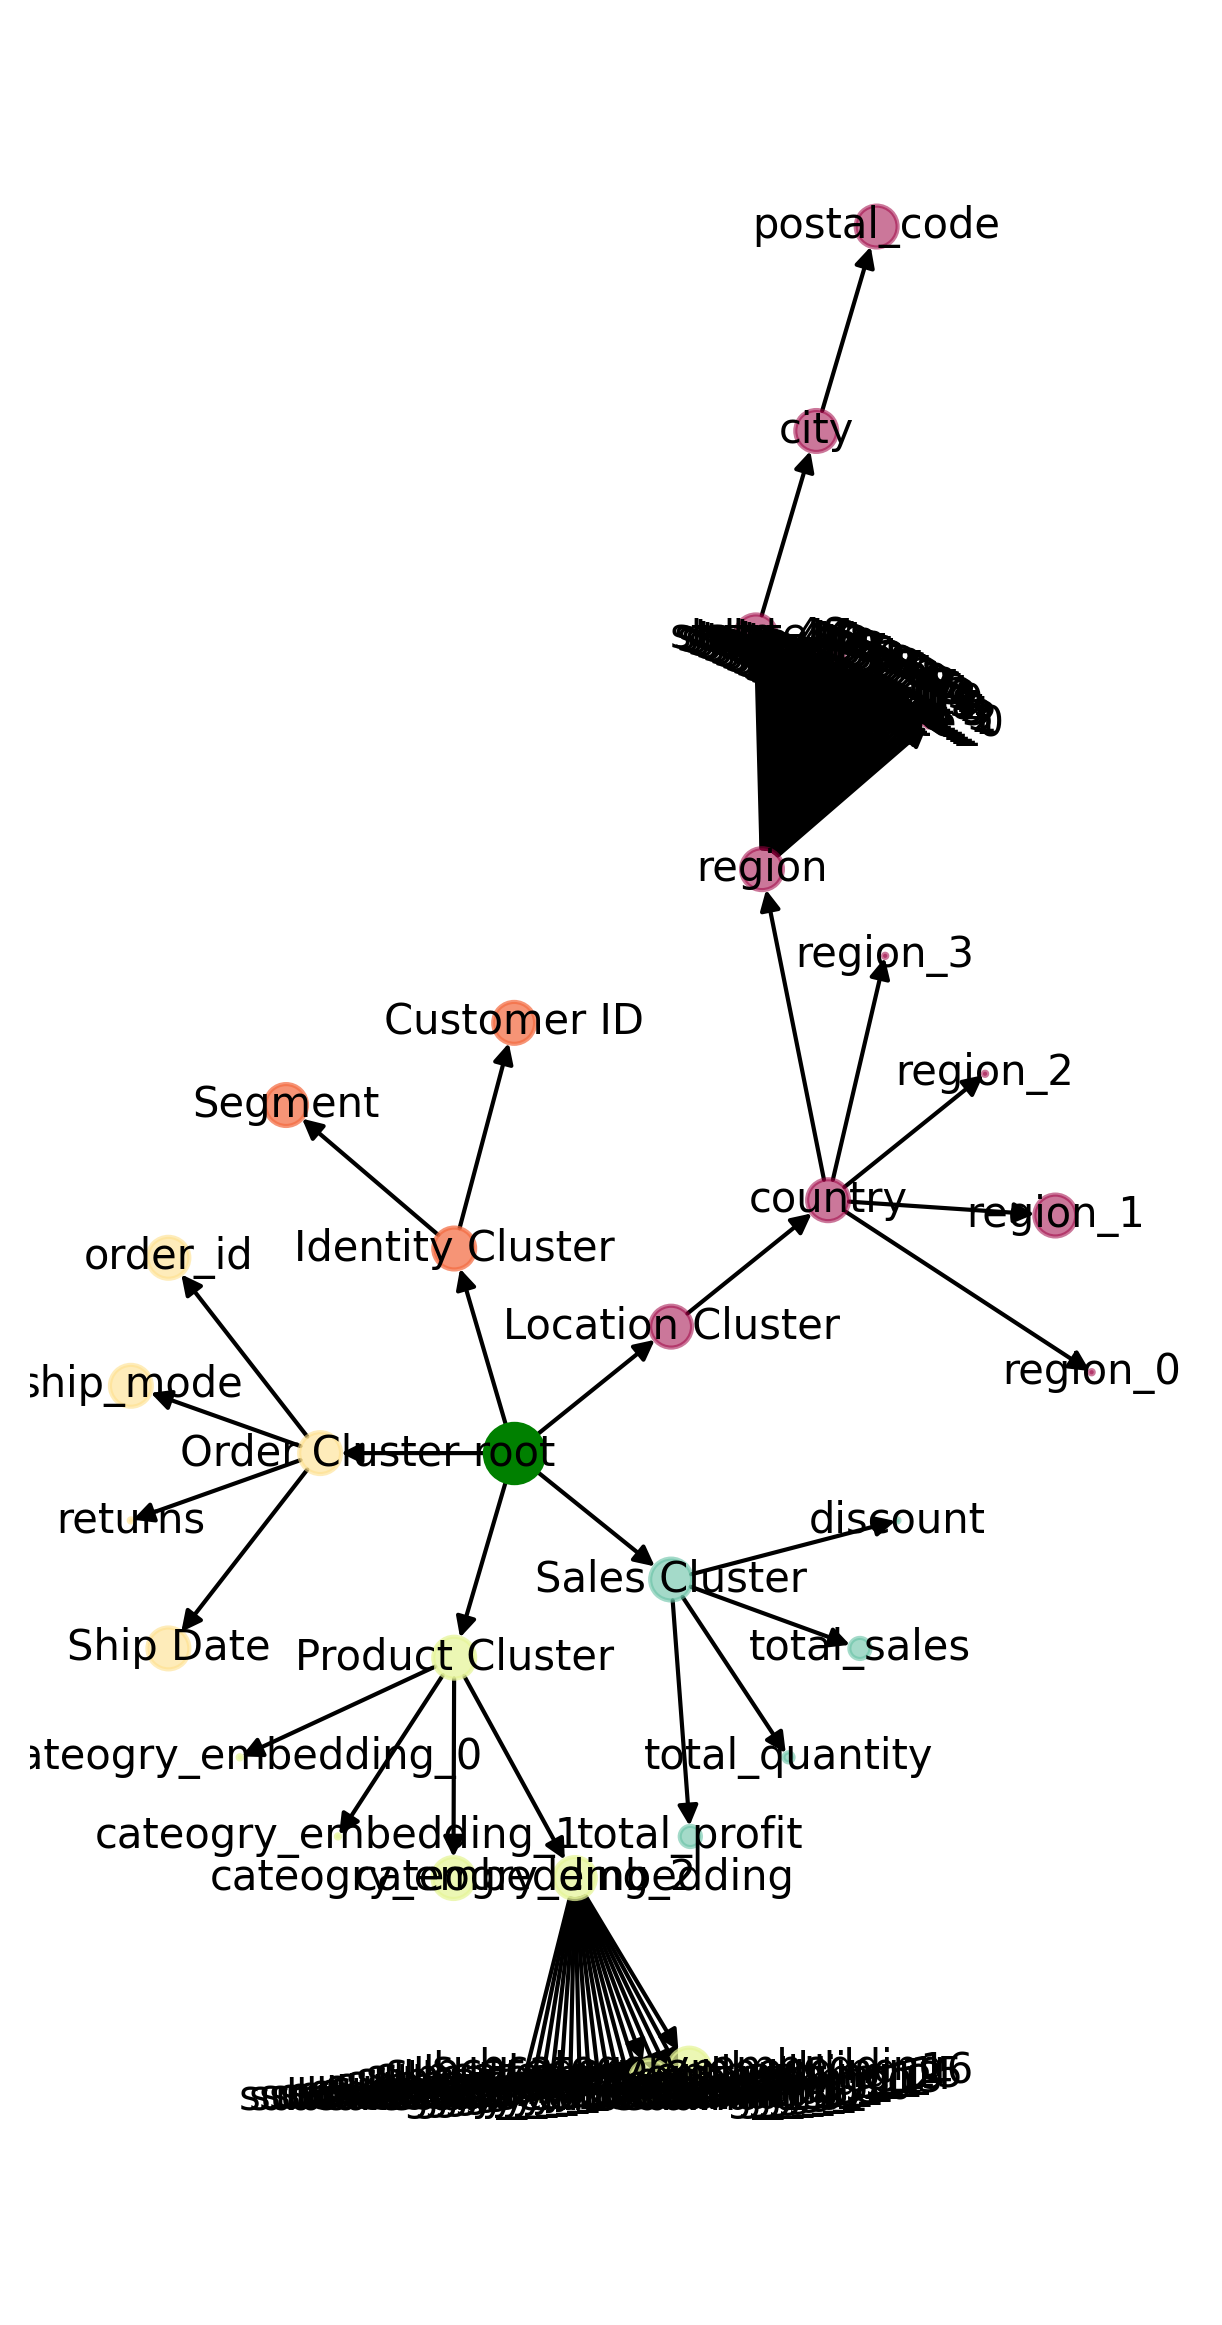
\includegraphics[width=0.5\textwidth]{images/base_model.png}
	\caption{\textit{The base R-K Model of the store sales data with appropriate filer and linker functions applied to the pipeline.}}
	\label{fig:base_model}
\end{figure}

\begin{figure}[H]
	\centering
        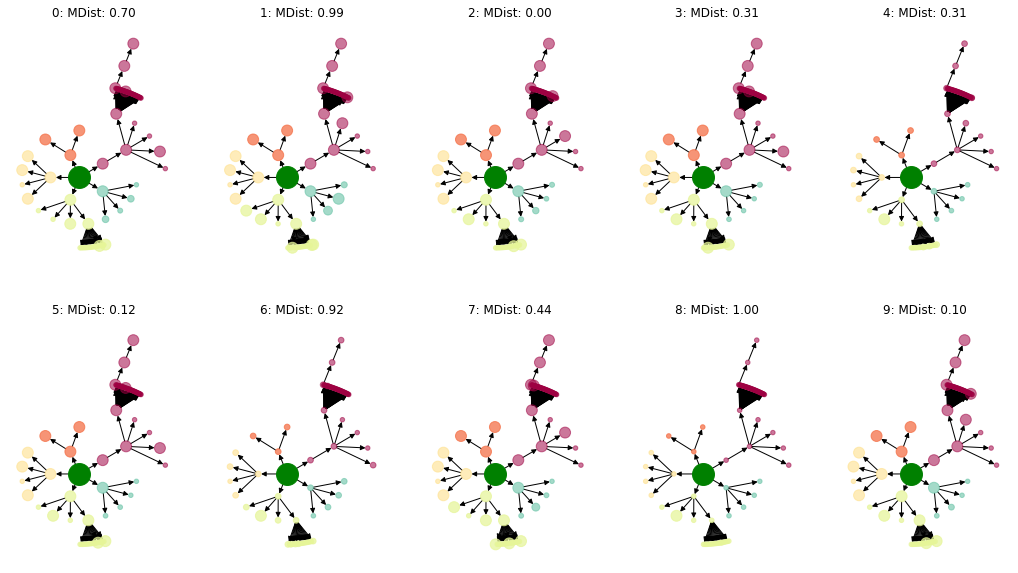
\includegraphics[width=0.5\textwidth]{images/store_sales_before_pipe_10.png}
	\caption{\textit{The first 10 events on an untuned network. M Dist is the normalized ( MinMaxScaled) Magnitudianal/Value distance of the data in data space as an extension of the Mahalanobis Distance formulation. Prior to training, the total average distance across graphs is 0.88. Topologically, there are no differences because no filters and/or linkages have been applied yet. The Topological Similarity measure in the above R-K Diagrams are all equal to 1. All deltas are derived from the distances of the values.}}
	\label{fig:store_sales_before_pipe}
\end{figure}

After filters and linkages have been applied, the untuned loss goes down from \textbf{0.88} to \textbf{0.78} with a preliminary Simple Child Linker and Range Filter applied to each node with the bounds [0,1].

\begin{figure}[H]
	\centering
        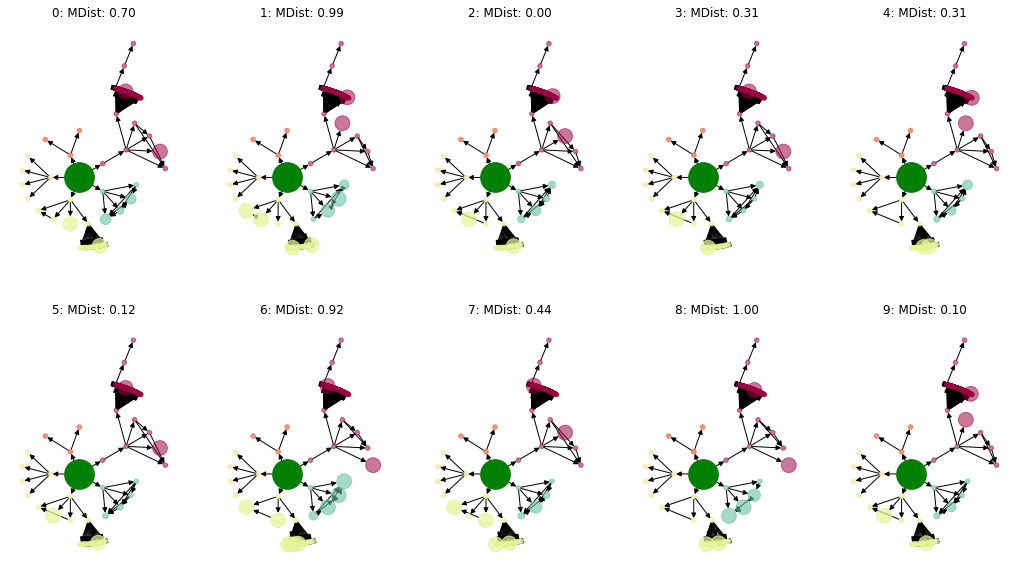
\includegraphics[width=0.5\textwidth]{images/store_sales_untuned_10.png}
	\caption{\textit{The first 10 events on an untuned network after filters and linkages applied. The initial guess was a RangeFilter of [0,1] applied to all nodes and a SimpleChildFilter with 0.5 as the initial starting point}}
	\label{fig:untuned_10}
\end{figure}


With filters and linkages, we get an improvement of \textbf{.1} from a pure value distances by introducing topological divergence through filters and linkers.

From a qualitative review, we can look event 6 and event 4, which according to Mahalanobis distance are quite different (.9 and .3) however topologically are quite similar. Conversely, 3 and 4 are very similar in Mahalanobis distance but very different topologically. This divergence would not normally be distinguishable using a traditional distance metric.

We can look at the individual transaction with more detail to get further understanding:

\begin{itemize}
\item Event 6 was a large purchase of $697.074$ dollars made in Houston. It was a highly discounted transaction and a multi-category purchase with 11 items.
\item Event 4 was a medium purchase of $21.376$ dollars made in Glendale. It had a $40$\% discount, was 5 items in a single category. 6 was very different to 4 in terms of Mahalanobis distance but very similar topologically. These are similar topologically because of the high discount rate, and the multi-category transaction type.
\item Event 3 was a smaller purchase of $3.928$ dollars made in New York. A $20$\% discount was applied and it was a single category purchase. Thus, Event 3 was very similar to event 4 in terms of Mahalanobis distance but very different topologically. This was very different topologically to Event 4, because unlike event 4; event 3 was a single item purchase.
\end{itemize}

In conclusion, using our loss function defined in \hyperref[sec:rk_distance]{Measuring R-K Distance}, we find that the average distance between R-K Models is \textbf{0.22}, and inversely, our similarity is \textbf{0.78} after applying filters and linkers. Before filters and linkers, topological distances across the models are 0. After filters and linkages, topological distances are 0.2 unweighted. Emergent properties from the data begin to form at this stage, however, to improve the results, we applied optimization and tuning of hyper-parameters via Machine Learning algorithms such that the appropriate weights to apply to the filters and maximize divergence across R-K Diagrams are learned automatically by applying combinatorial machine learning to the data via an implementation of Facebook's Nevergrad.\cite{a2020_nevergrad}

\subsection{Training The Pipeline}

In order to maximize divergence across R-K Diagrams, we trained our models using Facebook's Nevergrad \cite{a2020_nevergrad} optimizers. Thus, as demonstrated in the below sections, by providing an objective function and iterating over the various R-K models in a stochastic batch, we were able to reduce total loss of the set from \textbf{0.78} to \textbf{0.7}.

This gets us closer to providing a unique topological signatures across R-K Diagrams post training. This post-trained R-K Pipeline, could in theory be utilized across live stream data, to provide unique topological structures to incoming data from a similar dataset. This analysis is merely the beginning of optimization techniques that are possible with the R-K toolkit. Our goal for the following section is to show the potential of R-K Diagrams and Machine Learning, with the expectations that the methodology and implementation will improve with future research.

The loss history can be seen below and the description of how this loss function was obtained can be seen in the next sections.

\begin{figure}[H]
	\centering
        
\includegraphics[width=0.5\textwidth]{images/loss_over_time.png}
	\caption{\textit{Loss function over 1000 iterations}}
	\label{fig:loss_func}
\end{figure}

\subsubsection{Objective Function}
\label{sec:ObjectiveFunction}

We define an objective function as the following:

\begin{equation}
\frac{\sum^{n}_{i=0}\sum^{n}_{j=0}d(g_{i}, g_{j})}{ \frac{n!}{2(n-2)!}}
\end{equation}

The goal of the objective function, as defined above, is to maximize divergence across R-K Diagrams by minimizing the similarity across diagrams. This is determined through a distance function defined in the \hyperref[sec:rk_distance]{Measuring R-K Distance} subsection, which takes into account topological and magnitudal similarities across R-K Diagrams using a weighted distance function. We chose an even distribution of $[0.5, 0.5]$ for $w$ as a prior, as there is no reason to bias the weights apriori.

Over iteration of $\theta$, we will attempt to minimize the overall loss. Assuming an infinite number of iterations, we would hope that we maximize divergence across R-K Diagrams such that no R-K Diagram is exactly the same except for the same data, which would deterministically produce the same R-K Diagram.

The objective function provided above has large scope for future improvements and research, as ultimately the goal embedding the data into an R-K Diagram would be to maximize topological differences across differences in the shape of the data, and minimize differences of R-K Diagrams across similarity in attributes.

\subsubsection{Optimizer}
\label{sec:Optimizer}

Because topological distance functions do not exhibit continuous gradients we employed a gradient free optimization using Nevergrad. \cite{a2020_nevergrad}. NGOpts is an optimizer built by Facebook and the default suggested optimizer by Facebook. We ran with 5 max workers (parallelization) and a budget (number of allowed evalautions) of 1000.

\subsubsection{Post Training Results (Pre-Compression)}

The final results post training resulted in a loss of \textbf{0.825}. The diagrams post training are shown below:

\begin{figure}[H]
	\centering
        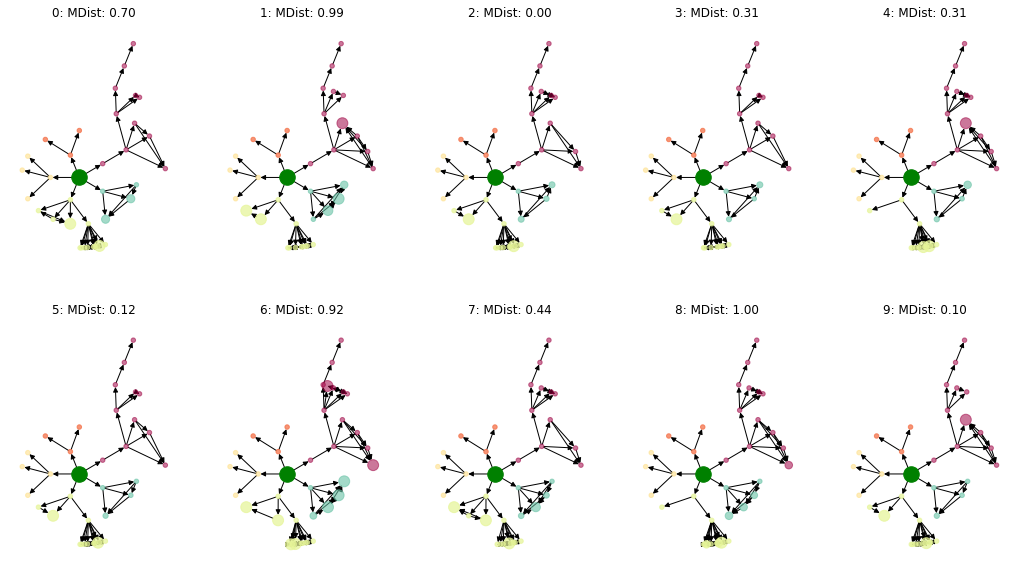
\includegraphics[width=0.5\textwidth]{images/store_sales_trained_data.png}
	\caption{\textit{Tuned R-K Diagrams (Pre-Compression)}}
	\label{fig:store_sales_trained_data}
\end{figure}

As you can see in the above, by maximizing distances across R-K Diagrams, we can see distinct topological signatures across events. This allows us to perform a variety of different methods of analysis later on, such as classification (given an R-K diagram, assign a label), estimation (given an R-K Diagram, estimate some value based), or other ML related techniques. There are many possibilities, if one considers the R-K Model as an input layer to a model.

In the case above, we can embed the R-K Diagrams in a 2D space and cluster them based upon attributes of the R-K Diagram.

\subsubsection{Isometric Compression}

Unlike standard dimensionality reduction techniques, compression techniques applied to the R-K Diagrams do not lose resolution in the data and can also maintain a consistent number of dimensions (2 or 3) of diagrams regardless of the number of model dimensions. This makes it far easier to evaluate models in higher dimensional space qualitatively without data loss and is one of the primary advantages to the pipeline.

We used the steps outlined in \hyperref[subsec:compression]{Isometric Compressions, Inverse Function, and Decompression} for graph compression. We used a limited compression technique via a 1 degree leaf compression technique, which compressed all 1 degree or ``unlinked'' leafs into a single compressed leaf branching from the same parent. The steps are maintained internally so that the original structural graph can be reconstructed from compressed version, thereby providing the inverse transformation. With future research, we may employ various other compressible techniques (outlined in 4.5.9) to the store sales data to achieve better results.

\begin{figure}[H]
	\centering
        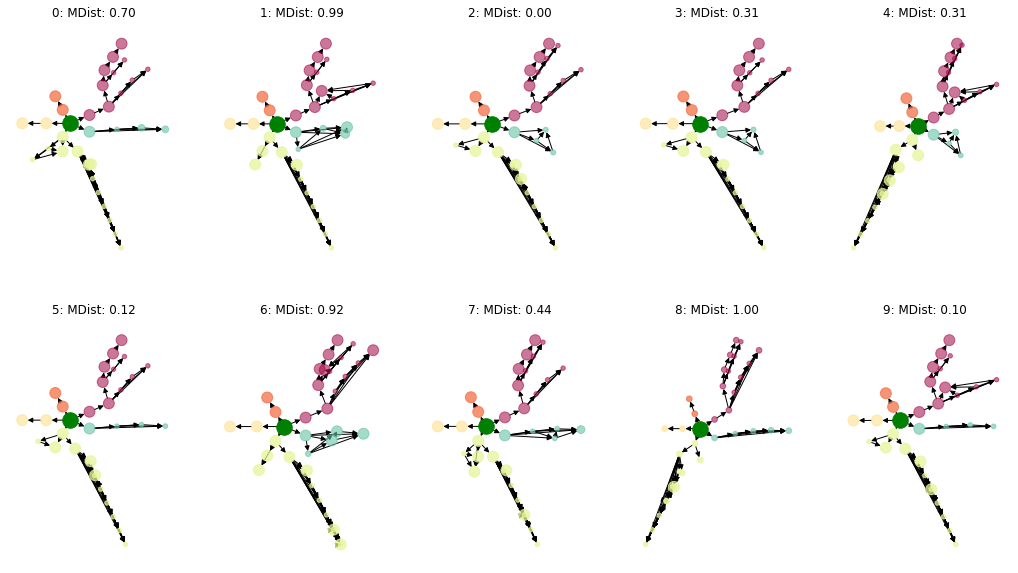
\includegraphics[width=0.5\textwidth]{images/compressed_store_sales.png}
	\caption{\textit{Isometrically Compressed R-K Diagrams}}
	\label{fig:compresseion_example_fig}
\end{figure}


\subsubsection{ML over R-K Diagrams for Variant Use Cases}
\label{sec:classification}

By generating distinct R-K Diagrams, it is possible to employ many standard Machine Learning algorithms for numerous use cases such as classification, clustering, segmentation, and identification. For example, we could use cluster the R-K Diagrams into segments. Such segments could then be used to optimize store operations or sales across the data.One such classification example has been demonstrated below using a tSNE based localization and clustering technique. This technique provides a 2D embedding of the isometrically compressed R-K diagrams using the information derived from R-K distance and similarity measures via a comparison of Magnitudinal/Value Distance and Topological Distance between the various purchase events represented by their corresponding R-K Diagrams. A sample demonstration of the above can be seen in figure \ref{fig:tsne} for reference.

 \begin{figure}[h]
	\centering
       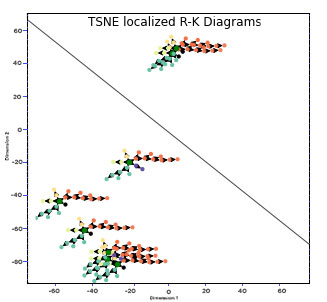
\includegraphics[width=0.5\textwidth]{images/tSNE LocalizedRKDiagrams.jpg}
  \caption{\textit{tSNE localized R-K Diagrams with ML Based clustering via measures of R-K distance between various events with tSNE Dimension 1 and tSNE Dimension 2 plotted on the x \& y axis respectively.}}
 \label{fig:tsne}
\end{figure}

Other use cases such as classification also become possible. The classification use case is used in LIGO (described below), which used R-K Diagrams to describe Binary Merger Event Classifications. Since a pipeline is event level, stream data can be fed into the pipeline to generate new R-K diagram, with a single event generating a unique topological signature. As more data comes in, these models can be refined to provide greater sensitivity to topological differences.


\subsubsection{Conclusion and Future Work}

In conclusion, the store sales dataset has demonstrated a novel approach using event driven Topological Graph Theory Analysis on a canonical and standard, non-scientific dataset. It proves our first case of generalizability outside the initial models made for the LIGO analysis.

Future work can be done to improve the R-K pipeline and algorithms such that more distance and accurate signatures are derived from the store sales data. Further more, applying the signatures to various use cases such as classification or identification would be a valuable exercise and is in scope for future papers.
